\documentclass[12pt, a4paper]{article}

% Acentuação
\RequirePackage[T1]{fontenc}
\RequirePackage[utf8]{inputenc}

% Configurando as margens
\usepackage[top = 2cm, bottom = 2cm, left = 3cm, right = 3cm]{geometry}
% Indentação do parágrafo
\setlength{\parindent}{2cm}
% Espaçamento entre parágrafo e texto
\setlength{\parskip}{1em}
% Espaçamento entre linhas
\renewcommand{\baselinestretch}{1.5}
% Identar o primeiro parágrafo das seções
\usepackage{indentfirst}
% Para usar símbolos como >=
\usepackage{amssymb}
% Para colocar texto entre $$ com \text{oi}
\usepackage{amsmath}
% Para usar listas com estilos específicos
\usepackage{enumerate}
% Para utilizar imagens
\usepackage{graphicx}

\renewcommand{\figurename}{Figura}

\begin{document}

	\input{Título.tex}

	\section{Pré-dimensionamento de lajes maciças}
	Para o pré-dimensionamento da espessura das lajes maciças, deve-se utilizar a seguinte equação: $$h=\frac{lx}{40}$$ 

Onde $h$ é a altura da laje em $cm$ e $lx$ é menor medida em $cm$ de um dos lados da laje.

As dimensões mínimas especificadas na \textbf{NBR 6118/14} são, em $cm$:

\begin{itemize}
	\item $h \geqslant 7$ para lajes de cobertura (não em balanço);
	\item $h \geqslant 8$ para lajes de piso (não em balanço);
	\item $h \geqslant 10$ para lajes em balanço;
	\item $h \geqslant 10$ para estacionamento para veículos até 30 $kN$;
	\item $h \geqslant 12$ para estacionamento para veículos com mais de 30 $kN$.
\end{itemize}

Tentar sempre arredondar para o inteiro superior mais próximo, a fim de facilitar a confecção da forma da laje, sempre se atentando ao mínimo exigido na norma.

	\section{Pré-dimensionamento de pilares maciços}
	Os pilares são pré-dimensionados para atuarem com uma \textbf{tensão de serviço} ($\sigma$) de $1,0$ a $1,5$ $kN/cm^2$ submetidos a uma ação de $10$ a $12$ $kN/m^2$ por pavimento (carga por pavimento).

Deve-se considerar os seguintes itens para a obtenção das medidas de seção dos pilares:

\begin{itemize}
	\item Espessura dos blocos das paredes adjacentes ($19$ $cm$ para pilares externos e $14$ $cm$ para internos);
	\item Tensão de serviço;
	\item Carga por pavimento;
	\item Número de pavimentos.
\end{itemize}

A carga na base do pilar é o produto: $$F_bi = A_{inf}i \cdot F_{pav} \cdot N_{pav}$$

Onde $F_bi$ é a força na base do pilar $i$ em $kN$, $A_{inf}i$ é a área de influência das lajes adjacentes ao pilar $i$ em $m^2$, $F_{pav}$ é a carga por pavimento em $kN/m^2$ e $N_{pav}$ é o número de pavimentos.

As dimensões da área de influência das lajes em um determinado pilar são montadas a partir da metade da distância até os pilares adjacentes, como na seguinte imagem:

\begin{figure}[h]
	\begin{center}
    	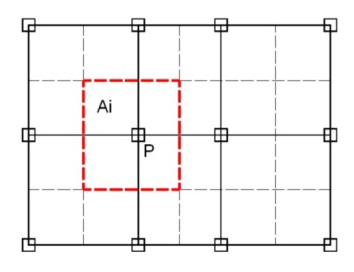
\includegraphics[width=0.5\textwidth]{Pre-dimensionamento-pilares-macicos/Imagens/Area-de-influencia-das-lajes-nos-pilares.jpg}
    	\caption{Área de influência \textit{i} das lajes adjacentes em um pilar \textit{P}.}
	\end{center}
\end{figure}

Obtida a carga na base do pilar, pode-se obter a área da seção pelo quociente, lembrando-se que $\sigma = \lim_{\Delta A \rightarrow 0} \frac{\Delta F}{\Delta A}$, portanto:

$$A_i = \frac{F_bi}{\sigma}$$

Onde $A_i$ é a área da seção transversal do pilar $i$ em $cm^2$, $F_bi$ é a força na base do pilar $i$ em $kN$ e $\sigma$ é a tensão de serviço em $kN/cm^2$.

A \textbf{área mínima} de seção transversal para pilares é de $360$ $cm^2$ e deve ser adotada caso a equação acima dê um valor inferior.

Obtida a área da seção, pode-se finalmente obter a estimativa das dimensões do pilar. Tem-se previamente uma das dimensões (19 $cm$ para pilares externos e 14 $cm$ para internos) e pode-se encontrar a restante a partir da equação da área do retângulo $(base \cdot altura)$ para pilares retangulares.

A nomenclatura das dimensões dos pilares em projetos de estruturas (plantas) é \textbf{Pi (largura x altura)}, por exemplo, \textbf{P5 (19 x 35)}.

	\section{Cargas nas lajes}
	Há basicamente dois tipos de cargas verticais em lajes maciças, \textbf{cargas permanentes} e \textbf{cargas acidentais}. A primeira sempre existirá na vida útil do edifício, a segunda é decorrente da utilização do ambiente. As cargas acidentais são tabeladas e definidas pela \textbf{NBR 6120}.

As cargas permanentes podem ser subdivididas em quatro, sendo:

\begin{itemize}

	\item \textbf{Peso próprio da laje (g1)}:
	
		$$g1=\gamma_c \cdot h$$

		Onde $\gamma_c$ é o peso específico da laje em $kN/m^3$ e $h$ é a altura da laje em $m$. Portanto, a unidade de $g1$ é $kN/m^2$, ficando em função da área da laje.
		
	\item \textbf{Revestimento (g2)}:
		Considera-se geralmente de $1,0$ a $1,5$ $kN/m^2$.
		
	\item \textbf{Enchimento (g3)}:
		Encontra-se geralmente no teto de banheiros, onde há passagem da tubulação.
		
		$$g3=\gamma_e \cdot h_e$$
		
		Onde $\gamma_e$ é o peso específico do enchimento em $kN/m^3$ e $h_e$ é a altura do enchimento em $m$. Portanto, a unidade de $g3$ é $kN/m^2$, ficando em função da área da laje.
		
	\item \textbf{Alvenaria direta sobre a laje (g4)}:
		Consiste na consideração da influência das paredes sobre a laje.
		
		$$g4=\frac{\gamma_a \cdot V_a}{lx \cdot ly}$$
		
		Onde $\gamma_a$ é o peso específico da alvenaria em $kN/m^3$, $V_a$ é o volume da alvenaria em $m^3$, $lx$ e $ly$ são o menor e maior vão da laje, respectivamente, em $m$. Portanto, a unidade de $g4$ é $kN/m^2$, ficando em função da área da laje.		
		
\end{itemize}

Alguns exemplos de cargas acidentais em edifícios (NBR 6120):

\begin{itemize}
	\item Dormitório, sala, cozinha e banheiro ($1,5$ $kN/m^2$);
	\item Despensa, área de serviço ($2,0$ $kN/m^2$);
	\item Varanda ($3,0$ $kN/m^2$).
\end{itemize}

Conhecendo-se as cargas permanentes e acidentais, considera-se a carga final na laje ($P$) como: $$P=P_{pe}+P_{ac}=(g1+g2+g3+g4)+P_{ac}$$

Onde $P_{pe}$ é a carga permanente total e $P_{ac}$ é a carga acidental do ambiente.
A carga final é utilizada para definir o carregamento nas vigas adjacentes às lajes.	

	\section{Pré-dimensionamento de vigas maciças}
	Para o pré-dimensionamento da altura de vigas, deve-se observar o número de apoios na qual ela está sujeita. Para obtenção dessa altura, deve-se utilizar as seguintes equações:

\begin{itemize}
	\item Para \textbf{vigas contínuas} com mais de dois apoios, subdivide-se a viga em vigas menores, portanto:

		$$h=c  \cdot \frac{L}{10}$$
		Onde $h$  é a altura da viga, $L$ é o comprimento do trecho e $c$ é 0,75 para vigas nas extremidades e 0,7 para as demais. Adota-se a maior altura encontrada para toda a seção transversal.

	\item Para \textbf{vigas em balanço}, temos:

		$$h=\frac{L}{5}$$
		Onde $h$ é a altura da viga e $L$ seu comprimento.

	\item Para \textbf{vigas biapoiadas}, temos:
		
		$$h=\frac{L}{10}$$
		Onde $h$ é a altura da viga e $L$ seu comprimento.
\end{itemize}

Recomenda-se \textbf{não pré-dimensionar} vigas com menos de 25 $cm$ de altura.

Deve-se atentar, entretanto, que para lajes onde há a necessidade da passagem de tubulações, é necessário ajustar a altura da viga. Por exemplo, o teto de banheiros precisa de tubulações, deve-se considerar a espessura da laje do banheiro e a espessura do local onde ficará a tubulação. Para que as vigas não fiquem aparentes, além do usual método de adotar \textbf{alturas de 5 em 5 $cm$}  para facilitar a montagem da forma, deve-se \textbf{cobrir toda essa espessura onde há a tubulação + laje}. Isso é muito importante.

Adota-se $bw$ $\geqslant$ 14 $cm$ , podendo ser $\geqslant$ 12 $cm$ em casos especiais.

	\section{Cargas nas vigas}
	As cargas verticais nas vigas são:

\begin{itemize}
	\item \textbf{Peso próprio da viga}:

		$$g_{viga}=\gamma_c\cdot bw\cdot h$$

		Onde $g_{viga}$ é o peso próprio da viga em $kN/m^3$, $\gamma_c$ é o peso específico do concreto armado, $bw$ é a largura da seção transversal da viga em $m$ e $h$ é a altura da seção transversal da viga em $m$.

	\item \textbf{Alvenaria sobre a viga}:

		$$g_{alv}=\gamma_{alv}\cdot h\cdot e$$

		Onde $g_{alv}$ é o peso da alvenaria sobre a viga em $kN/m$, $\gamma_{alv}$ é o peso específico da alvenaria que está sobre a viga em $kN/m^3$, $h$ é a altura da parede em $m$ e $e$ é a espessura da parede em $m$.

	\item \textbf{Carga das lajes sobre as vigas}:

		Sendo $P$ a carga nas lajes, devemos distribuir geometricamente $P$ para as vigas. Isso é feito analisando os apoios da laje, pois apoios engastados geralmente recebem mais carga. O primeiro passo é encontrar a área de influência das lajes para as vigas em função dos seus apoios, como na seguinte figura:

	A carga $px$ e $py$, obviamente, serão menores que a carga $P$, entretanto, suas unidades são diferentes. $P$ está em função da área da laje, já $px$ e $py$ estão em função do comprimento da viga.


\end{itemize}

	\section{Cálculo da armadura longitudinal em vigas sob flexão normal}
	O cálculo da quantidade de armadura longitudinal para seções transversais retangulares, conhecidos a resistência do concreto ($f_{ck}$), a largura da seção ($b_w$), a altura útil ($d$) e o tipo de aço ($f_{yd}$ e $\epsilon_{yd}$), é feito de maneira simples, a partir do equilíbrio das forças atuantes na seção. Será estudada a flexão normal pura e simples, representada pelos domínios 2, 3, 4 e 4a.

Considerando o seguinte problema: Conhecidos $f_{ck}$, $b_w$, $d$, tipo de aço ($f_{yd}$ e $\epsilon_{yd}$) e o momento de cálculo $M_d$ ($M_d=1,4\cdot M_k$), determinar a área da armadura longitudinal necessária, ($A_s$) para que uma viga de concreto armado e de seção transversal retangular resista a esse momento fletor.

*Inserir figura
\begin{itemize}
	\item \textbf{Equilíbrio das forças atuantes normais à seção transversal}: Como não há força externa, a força atuante no concreto ($F_c$), deve ser igual à força atuante na armadura ($F_s$):
		\begin{equation}
			\label{equacao-equilibrio-forcas}
			\sum F=0\rightarrow F_s-F_c=0\rightarrow F_s=F_c
		\end{equation}

	\item \textbf{Equilíbrio dos momentos}: O momento das forças internas em relação a qualquer ponto (no caso, em relação ao ponto $C.G.$ da armadura) deve ser igual ao momento externo de cálculo:
		\begin{equation}
			\label{equacao-equilibrio-momentos}
			\sum M=M_d\rightarrow M_d=F_c\cdot z
		\end{equation}
\end{itemize}

Das Equações~\eqref{equacao-equilibrio-forcas} e~\eqref{equacao-equilibrio-momentos}, tem-se:
\begin{equation}
	\label{equacao-momento-de-calculo1}
	M_d=F_s\cdot z
\end{equation}

\begin{itemize}
	\item \textbf{Posição da linha neutra ($x$)}: Conhecendo a posição da linha neutra, é possível saber o domínio em que a peça está trabalhando e calcular a resultante das tensões de compressão no concreto ($F_c$) e o braço de alavanca ($z$).
		\begin{equation}
			\label{equacao-resultante-fc}
			F_c=(0,85\cdot f_{cd})\cdot(b_w)\cdot(0,8\cdot x)
		\end{equation}
		\begin{equation}
			\label{equacao-z}
			z=d-0,4\cdot x
		\end{equation}
\end{itemize}

Colocando $F_c$ e $z$ na Equação~\eqref{equacao-equilibrio-momentos}, tem-se:
\begin{equation}
	M_d=F_c\cdot z=(0,85\cdot f_{cd}\cdot b_w\cdot0,8\cdot x)\cdot(d-0,4\cdot x)=b_w\cdot f_{cd}\cdot0,68\cdot x\cdot(d-0,4\cdot x)
\end{equation}

Ou, ainda:
\begin{equation}
	\label{equacao-momento-de-calculo}
	M_d=(0,68\cdot x\cdot d-0,272\cdot x^2)\cdot b_w\cdot f_{cd}
\end{equation}

Resolvendo a Equação~\eqref{equacao-momento-de-calculo} obtém-se $x$, o qual define a posição da linha neutra, que é fundamental para a solução do problema proposto. Nota-se que a variação de $x$ não é linear com o esforço solicitante $M_d$, mas segue um polinômio do segundo grau. Resolvendo a Equação~\eqref{equacao-momento-de-calculo} para $x$, tem-se:
\begin{equation}
	\label{equacao-linha-neutra1}
	x=1,25\cdot d\cdot\left(1\pm\sqrt{1-\frac{M_d}{0,425\cdot b_w\cdot f_{cd}\cdot d^2}}\right)
\end{equation}

Como a soma na Equação~\eqref{equacao-linha-neutra1} não tem sentido físico, tem-se, portanto:
\begin{equation}
	\label{equacao-linha-neutra}
	x=1,25\cdot d\cdot\left(1-\sqrt{1-\frac{M_d}{0,425\cdot b_w\cdot f_{cd}\cdot d^2}}\right)
\end{equation}

\begin{itemize}
	\item \textbf{Cálculo da área necessária de armadura ($A_s$)}: Com o valor de $x$ determinado, é possível encontrar $A_s$. A força na armadura ($F_s$) vem do produto da área de aço ($A_s$) pela tensão atuante no aço ($f_s$). Da Equação~\eqref{equacao-momento-de-calculo1}, tem-se $M_d/z=F_s=f_s\cdot A_s$, resultando em:
\end{itemize}
\begin{equation}
	\label{equacao-area-de-aco1}
	A_s=\frac{M_d}{z\cdot f_s}
\end{equation}

Admitindo que a peça esteja trabalhando no domínio 2 ou 3, para um melhor aproveitamento da armadura, tem-se $\epsilon_s\geqslant\epsilon_{yd}$, resultando na tensão de escoamento na armadura ($f_s=f_{yd}$); caso contrário, tira-se o valor de $\epsilon_s$ do diagrama de tensão \textit{versus} deformação do aço e calcula-se $f_s$. A Equação~\eqref{equacao-area-de-aco1} modifica-se:
\begin{equation}
	A_s=\frac{M_d}{z\cdot f_{yd}}
\end{equation}

	\section{Domínios de deformação}
	Obtido o valor de $x$ que define a posição (profundidade) da linha neutra, é possível verificar em que domínio a peça atingirá o Estado Limite Último. Na flexão simples, que está sendo considerada, os domínios possíveis são 2, 3 e 4. No início do domínio 2 tem-se $\epsilon_c=0$, e no final do domínio 4, $\epsilon_s=0$, que são as piores situações que podem ocorrer (um dos dois materiais não contribui na resistência). O melhor é que a peça trabalhe no domínio 3; o domínio 2 é aceitável; e o domínio 4 deve ser evitado. Cabe então a pergunta: Conhecido o momento e demais variáveis necessárias para resolver o problema, como saber se a seção está trabalhando no domínio 3 e se a armadura já atingiu a deformação de escoamento? É possível saber por meio da relação entre as deformações e a posição da linha neutra.

\begin{figure}[H]
	\begin{center}
	\caption{Domínios de deformação.}
    	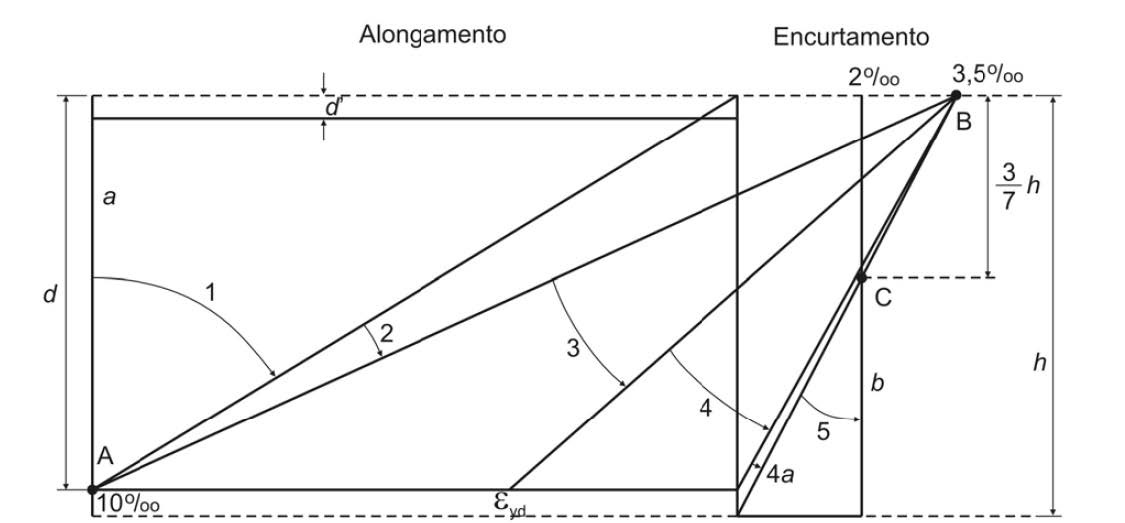
\includegraphics[width=\textwidth]{Dominios-de-deformacao/Imagens/Dominios-de-deformacao.jpg}
	\end{center}
\end{figure}

A linha neutra no domínio 1 está em ($-\infty<x\leqslant0$); no domínio 2 é necessário encontrar por semelhança de triângulos, já que foi considerada a hipótese de que as seções permanecem planas após as deformações. Ou seja:
$$\frac{x}{3,5\text{\textperthousand}}=\frac{d-x}{10\text{\textperthousand}}$$
$$10\text{\textperthousand}\cdot x=3,5\text{\textperthousand}\cdot d-3,5\text{\textperthousand}\cdot x$$

Isolando $x$, tem-se:
$$x=\frac{3,5\text{\textperthousand}\cdot d}{10\text{\textperthousand}+3,5\text{\textperthousand}}=0,259\cdot d$$

Portanto, a linha neutra do domínio 2 está em ($0<x\leqslant0,259\cdot d$). De maneira semelhante, para o domínio 3, tem-se:
\begin{equation}
	\label{equacao-dominio-3}
	\frac{x}{3,5\text{\textperthousand}}=\frac{d-x}{\epsilon_s}
\end{equation}

Pela Lei de Hooke ($\sigma=\text{E}\cdot\epsilon$) e pelo módulo de Young do aço ser de 210 $GPa$, o valor de $\epsilon_s$ (valor de deformação onde ocorre o início do escoamento do aço) depende do tipo de aço utilizado. O mais comum nas contruções de concreto armado é o aço CA-50. O número 50 diz que a tensão de escoamento desse aço é de 50 $kN/{cm}^2$. Aplicando a Lei de Hooke para esse aço, tem-se:
$$50\;\frac{kN}{{cm}^2}=21000\;\frac{kN}{{cm}^2}\cdot\epsilon_k$$
$$\epsilon_k=\frac{50\;\frac{kN}{{cm}^2}}{21000\;\frac{kN}{{cm}^2}}=2,38\text{\textperthousand}$$

O valor de $\epsilon_s=2,38\text{\textperthousand}/1,15=2,07\text{\textperthousand}$. Portanto, desenvolvendo e isolando $x$ na Equação~\eqref{equacao-dominio-3} para o aço CA-50, tem-se:
$$\frac{x}{3,5\text{\textperthousand}}=\frac{d-x}{2,07\text{\textperthousand}}$$
$$2,07\text{\textperthousand}\cdot x=3,5\text{\textperthousand}\cdot d-3,5\text{\textperthousand}\cdot x$$
$$x=\frac{3,5\text{\textperthousand}\cdot d}{2,07\text{\textperthousand}+3,5\text{\textperthousand}}=0,628\cdot d$$

Portanto, a linha neutra do domínio 3 está em ($0,259\cdot d<x\leqslant0,628\cdot d$). Para o domínio 4 e para o aço CA-50, a linha neutra está em ($0,628\cdot d<x\leqslant d$); no domínio 4a, está em ($d<x\leqslant h$) e por último, no domínio 5, está em ($h<x<\infty$).


\end{document}